\documentclass[1p]{elsarticle_modified}
%\bibliographystyle{elsarticle-num}

%\usepackage[colorlinks]{hyperref}
%\usepackage{abbrmath_seonhwa} %\Abb, \Ascr, \Acal ,\Abf, \Afrak
\usepackage{amsfonts}
\usepackage{amssymb}
\usepackage{amsmath}
\usepackage{amsthm}
\usepackage{scalefnt}
\usepackage{amsbsy}
\usepackage{kotex}
\usepackage{caption}
\usepackage{subfig}
\usepackage{color}
\usepackage{graphicx}
\usepackage{xcolor} %% white, black, red, green, blue, cyan, magenta, yellow
\usepackage{float}
\usepackage{setspace}
\usepackage{hyperref}

\usepackage{tikz}
\usetikzlibrary{arrows}

\usepackage{multirow}
\usepackage{array} % fixed length table
\usepackage{hhline}

%%%%%%%%%%%%%%%%%%%%%
\makeatletter
\renewcommand*\env@matrix[1][\arraystretch]{%
	\edef\arraystretch{#1}%
	\hskip -\arraycolsep
	\let\@ifnextchar\new@ifnextchar
	\array{*\c@MaxMatrixCols c}}
\makeatother %https://tex.stackexchange.com/questions/14071/how-can-i-increase-the-line-spacing-in-a-matrix
%%%%%%%%%%%%%%%

\usepackage[normalem]{ulem}

\newcommand{\msout}[1]{\ifmmode\text{\sout{\ensuremath{#1}}}\else\sout{#1}\fi}
%SOURCE: \msout is \stkout macro in https://tex.stackexchange.com/questions/20609/strikeout-in-math-mode

\newcommand{\cancel}[1]{
	\ifmmode
	{\color{red}\msout{#1}}
	\else
	{\color{red}\sout{#1}}
	\fi
}

\newcommand{\add}[1]{
	{\color{blue}\uwave{#1}}
}

\newcommand{\replace}[2]{
	\ifmmode
	{\color{red}\msout{#1}}{\color{blue}\uwave{#2}}
	\else
	{\color{red}\sout{#1}}{\color{blue}\uwave{#2}}
	\fi
}

\newcommand{\Sol}{\mathcal{S}} %segment
\newcommand{\D}{D} %diagram
\newcommand{\A}{\mathcal{A}} %arc


%%%%%%%%%%%%%%%%%%%%%%%%%%%%%5 test

\def\sl{\operatorname{\textup{SL}}(2,\Cbb)}
\def\psl{\operatorname{\textup{PSL}}(2,\Cbb)}
\def\quan{\mkern 1mu \triangleright \mkern 1mu}

\theoremstyle{definition}
\newtheorem{thm}{Theorem}[section]
\newtheorem{prop}[thm]{Proposition}
\newtheorem{lem}[thm]{Lemma}
\newtheorem{ques}[thm]{Question}
\newtheorem{cor}[thm]{Corollary}
\newtheorem{defn}[thm]{Definition}
\newtheorem{exam}[thm]{Example}
\newtheorem{rmk}[thm]{Remark}
\newtheorem{alg}[thm]{Algorithm}

\newcommand{\I}{\sqrt{-1}}
\begin{document}

%\begin{frontmatter}
%
%\title{Boundary parabolic representations of knots up to 8 crossings}
%
%%% Group authors per affiliation:
%\author{Yunhi Cho} 
%\address{Department of Mathematics, University of Seoul, Seoul, Korea}
%\ead{yhcho@uos.ac.kr}
%
%
%\author{Seonhwa Kim} %\fnref{s_kim}}
%\address{Center for Geometry and Physics, Institute for Basic Science, Pohang, 37673, Korea}
%\ead{ryeona17@ibs.re.kr}
%
%\author{Hyuk Kim}
%\address{Department of Mathematical Sciences, Seoul National University, Seoul 08826, Korea}
%\ead{hyukkim@snu.ac.kr}
%
%\author{Seokbeom Yoon}
%\address{Department of Mathematical Sciences, Seoul National University, Seoul, 08826,  Korea}
%\ead{sbyoon15@snu.ac.kr}
%
%\begin{abstract}
%We find all boundary parabolic representation of knots up to 8 crossings.
%
%\end{abstract}
%\begin{keyword}
%    \MSC[2010] 57M25 
%\end{keyword}
%
%\end{frontmatter}

%\linenumbers
%\tableofcontents
%
\newcommand\colored[1]{\textcolor{white}{\rule[-0.35ex]{0.8em}{1.4ex}}\kern-0.8em\color{red} #1}%
%\newcommand\colored[1]{\textcolor{white}{ #1}\kern-2.17ex	\textcolor{white}{ #1}\kern-1.81ex	\textcolor{white}{ #1}\kern-2.15ex\color{red}#1	}

{\Large $\underline{10_{96}~(K10a_{24})}$}

\setlength{\tabcolsep}{10pt}
\renewcommand{\arraystretch}{1.6}
\vspace{1cm}\begin{tabular}{m{100pt}>{\centering\arraybackslash}m{274pt}}
\multirow{5}{120pt}{
	\centering
	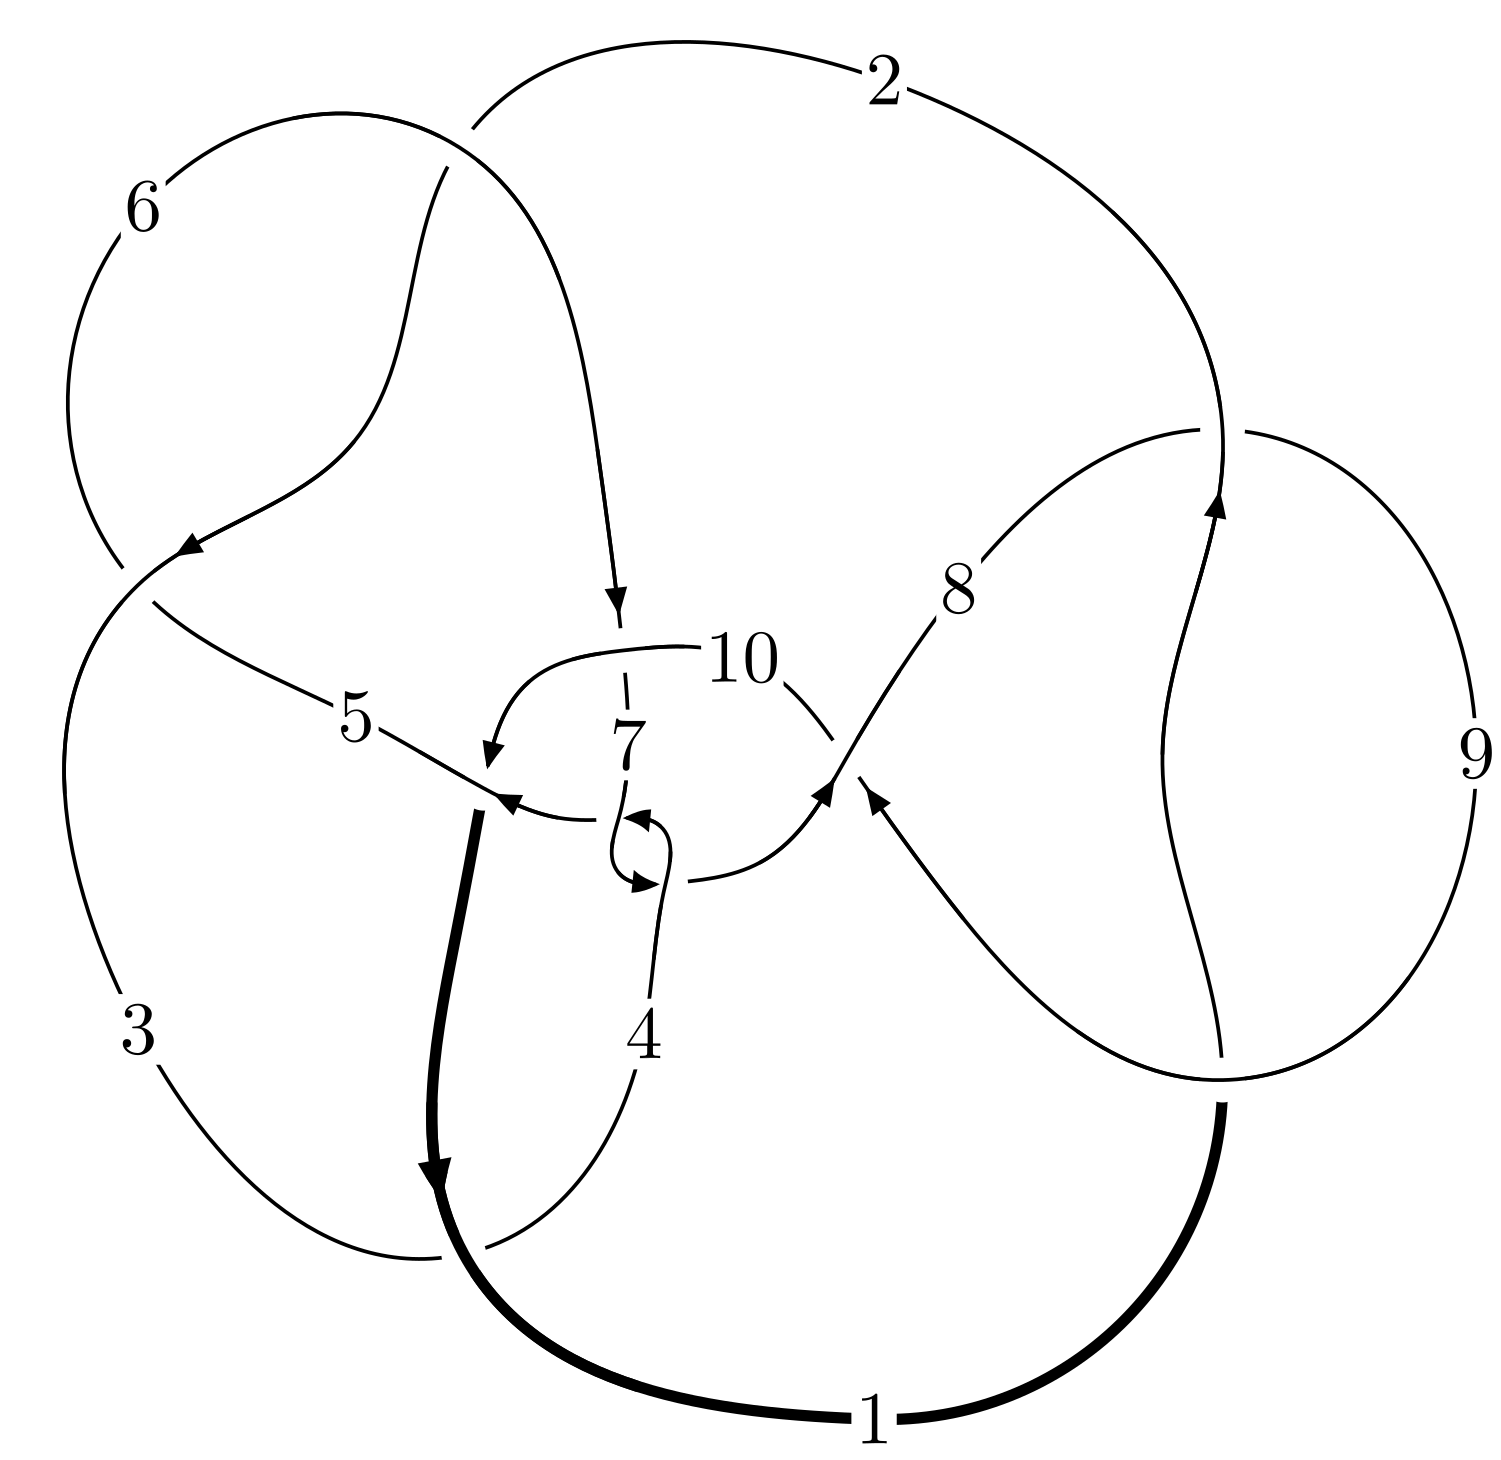
\includegraphics[width=112pt]{../../../GIT/diagram.site/Diagrams/png/180_10_96.png}\\
\ \ \ A knot diagram\footnotemark}&
\allowdisplaybreaks
\textbf{Linearized knot diagam} \\
\cline{2-2}
 &
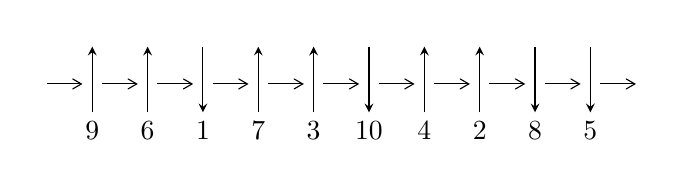
\begin{tikzpicture}[x=20pt, y=17pt]
	% nodes
	\node (C0) at (0, 0) {};
	\node (C1) at (1, 0) {};
	\node (C1U) at (1, +1) {};
	\node (C1D) at (1, -1) {9};

	\node (C2) at (2, 0) {};
	\node (C2U) at (2, +1) {};
	\node (C2D) at (2, -1) {6};

	\node (C3) at (3, 0) {};
	\node (C3U) at (3, +1) {};
	\node (C3D) at (3, -1) {1};

	\node (C4) at (4, 0) {};
	\node (C4U) at (4, +1) {};
	\node (C4D) at (4, -1) {7};

	\node (C5) at (5, 0) {};
	\node (C5U) at (5, +1) {};
	\node (C5D) at (5, -1) {3};

	\node (C6) at (6, 0) {};
	\node (C6U) at (6, +1) {};
	\node (C6D) at (6, -1) {10};

	\node (C7) at (7, 0) {};
	\node (C7U) at (7, +1) {};
	\node (C7D) at (7, -1) {4};

	\node (C8) at (8, 0) {};
	\node (C8U) at (8, +1) {};
	\node (C8D) at (8, -1) {2};

	\node (C9) at (9, 0) {};
	\node (C9U) at (9, +1) {};
	\node (C9D) at (9, -1) {8};

	\node (C10) at (10, 0) {};
	\node (C10U) at (10, +1) {};
	\node (C10D) at (10, -1) {5};
	\node (C11) at (11, 0) {};

	% arrows
	\draw[->,>={angle 60}]
	(C0) edge (C1) (C1) edge (C2) (C2) edge (C3) (C3) edge (C4) (C4) edge (C5) (C5) edge (C6) (C6) edge (C7) (C7) edge (C8) (C8) edge (C9) (C9) edge (C10) (C10) edge (C11) ;	\draw[->,>=stealth]
	(C1D) edge (C1U) (C2D) edge (C2U) (C3U) edge (C3D) (C4D) edge (C4U) (C5D) edge (C5U) (C6U) edge (C6D) (C7D) edge (C7U) (C8D) edge (C8U) (C9U) edge (C9D) (C10U) edge (C10D) ;
	\end{tikzpicture} \\
\hhline{~~} \\& 
\textbf{Solving Sequence} \\ \cline{2-2} 
 &
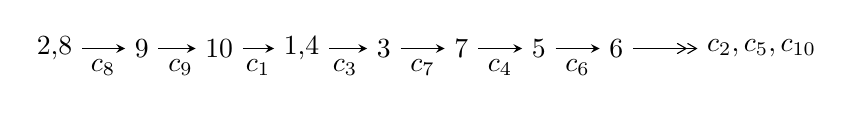
\begin{tikzpicture}[x=28pt, y=7pt]
	% node
	\node (A0) at (-1/8, 0) {2,8};
	\node (A1) at (1, 0) {9};
	\node (A2) at (2, 0) {10};
	\node (A3) at (49/16, 0) {1,4};
	\node (A4) at (33/8, 0) {3};
	\node (A5) at (41/8, 0) {7};
	\node (A6) at (49/8, 0) {5};
	\node (A7) at (57/8, 0) {6};
	\node (C1) at (1/2, -1) {$c_{8}$};
	\node (C2) at (3/2, -1) {$c_{9}$};
	\node (C3) at (5/2, -1) {$c_{1}$};
	\node (C4) at (29/8, -1) {$c_{3}$};
	\node (C5) at (37/8, -1) {$c_{7}$};
	\node (C6) at (45/8, -1) {$c_{4}$};
	\node (C7) at (53/8, -1) {$c_{6}$};
	\node (A8) at (9, 0) {$c_{2},c_{5},c_{10}$};

	% edge
	\draw[->,>=stealth]	
	(A0) edge (A1) (A1) edge (A2) (A2) edge (A3) (A3) edge (A4) (A4) edge (A5) (A5) edge (A6) (A6) edge (A7) ;
	\draw[->>,>={angle 60}]	
	(A7) edge (A8);
\end{tikzpicture} \\ 

\end{tabular} \\

\footnotetext{
The image of knot diagram is generated by the software ``\textbf{Draw programme}" developed by Andrew Bartholomew(\url{http://www.layer8.co.uk/maths/draw/index.htm\#Running-draw}), where we modified some parts for our purpose(\url{https://github.com/CATsTAILs/LinksPainter}).
}\phantom \\ \newline 
\centering \textbf{Ideals for irreducible components\footnotemark of $X_{\text{par}}$} 
 
\begin{align*}
I^u_{1}&=\langle 
-5272122 u^{17}+4798544 u^{16}+\cdots+51537967 b+28315457,\\
\phantom{I^u_{1}}&\phantom{= \langle  }38859701 u^{17}+11491400 u^{16}+\cdots+206151868 a-139434563,\\
\phantom{I^u_{1}}&\phantom{= \langle  }u^{18}+4 u^{16}+9 u^{14}- u^{13}+12 u^{12}-3 u^{11}+11 u^{10}-5 u^9+8 u^8+4 u^7+2 u^6+6 u^5+8 u^4+7 u^3+u^2+3 u+4\rangle \\
I^u_{2}&=\langle 
u^{14} a-2 u^{14}+\cdots-2 a-1,\;2 u^{14} a+2 u^{14}+\cdots+a^2+4 a,\\
\phantom{I^u_{2}}&\phantom{= \langle  }u^{15}- u^{14}+4 u^{13}-3 u^{12}+8 u^{11}-6 u^{10}+10 u^9-7 u^8+8 u^7-6 u^6+6 u^5-4 u^4+4 u^3-2 u^2+2 u-1\rangle \\
I^u_{3}&=\langle 
b-1,\;2 a+2 u+3,\;u^2+u+1\rangle \\
\\
\end{align*}
\raggedright * 3 irreducible components of $\dim_{\mathbb{C}}=0$, with total 50 representations.\\
\footnotetext{All coefficients of polynomials are rational numbers. But the coefficients are sometimes approximated in decimal forms when there is not enough margin.}
\newpage
\renewcommand{\arraystretch}{1}
\centering \section*{I. $I^u_{1}= \langle -5.27\times10^{6} u^{17}+4.80\times10^{6} u^{16}+\cdots+5.15\times10^{7} b+2.83\times10^{7},\;3.89\times10^{7} u^{17}+1.15\times10^{7} u^{16}+\cdots+2.06\times10^{8} a-1.39\times10^{8},\;u^{18}+4 u^{16}+\cdots+3 u+4 \rangle$}
\flushleft \textbf{(i) Arc colorings}\\
\begin{tabular}{m{7pt} m{180pt} m{7pt} m{180pt} }
\flushright $a_{2}=$&$\begin{pmatrix}0\\u\end{pmatrix}$ \\
\flushright $a_{8}=$&$\begin{pmatrix}1\\0\end{pmatrix}$ \\
\flushright $a_{9}=$&$\begin{pmatrix}1\\- u^2\end{pmatrix}$ \\
\flushright $a_{10}=$&$\begin{pmatrix}u^2+1\\- u^2\end{pmatrix}$ \\
\flushright $a_{1}=$&$\begin{pmatrix}- u\\u^3+u\end{pmatrix}$ \\
\flushright $a_{4}=$&$\begin{pmatrix}-0.188500 u^{17}-0.0557424 u^{16}+\cdots+0.154930 u+0.676368\\0.102296 u^{17}-0.0931070 u^{16}+\cdots-0.813721 u-0.549410\end{pmatrix}$ \\
\flushright $a_{3}=$&$\begin{pmatrix}-0.166761 u^{17}-0.0607885 u^{16}+\cdots+0.283272 u+1.04603\\0.0148237 u^{17}-0.207715 u^{16}+\cdots-0.870244 u-0.939258\end{pmatrix}$ \\
\flushright $a_{7}=$&$\begin{pmatrix}0.234815 u^{17}+0.0148237 u^{16}+\cdots-0.790765 u-0.165801\\-0.0607885 u^{17}+0.189164 u^{16}+\cdots+1.54632 u+0.667045\end{pmatrix}$ \\
\flushright $a_{5}=$&$\begin{pmatrix}-0.373129 u^{17}-0.128980 u^{16}+\cdots+0.922103 u+1.59149\\0.128980 u^{17}-0.289335 u^{16}+\cdots-2.71088 u-1.49252\end{pmatrix}$ \\
\flushright $a_{6}=$&$\begin{pmatrix}0.137352 u^{17}+0.102296 u^{16}+\cdots-0.248070 u-0.401663\\-0.0557424 u^{17}+0.123431 u^{16}+\cdots+1.24187 u+0.754001\end{pmatrix}$\\&\end{tabular}
\flushleft \textbf{(ii) Obstruction class $= -1$}\\~\\
\flushleft \textbf{(iii) Cusp Shapes $= -\frac{23479367}{51537967} u^{17}-\frac{127343919}{206151868} u^{16}+\cdots+\frac{657635827}{206151868} u+\frac{414460539}{51537967}$}\\~\\
\newpage\renewcommand{\arraystretch}{1}
\flushleft \textbf{(iv) u-Polynomials at the component}\newline \\
\begin{tabular}{m{50pt}|m{274pt}}
Crossings & \hspace{64pt}u-Polynomials at each crossing \\
\hline $$\begin{aligned}c_{1},c_{8}\end{aligned}$$&$\begin{aligned}
&u^{18}+4 u^{16}+\cdots-3 u+4
\end{aligned}$\\
\hline $$\begin{aligned}c_{2},c_{4},c_{5}\\c_{7}\end{aligned}$$&$\begin{aligned}
&u^{18}-2 u^{17}+\cdots- u+1
\end{aligned}$\\
\hline $$\begin{aligned}c_{3},c_{6}\end{aligned}$$&$\begin{aligned}
&4(4 u^{18}-6 u^{17}+\cdots+u+1)
\end{aligned}$\\
\hline $$\begin{aligned}c_{9}\end{aligned}$$&$\begin{aligned}
&u^{18}+8 u^{17}+\cdots- u+16
\end{aligned}$\\
\hline $$\begin{aligned}c_{10}\end{aligned}$$&$\begin{aligned}
&u^{18}+3 u^{17}+\cdots+120 u+32
\end{aligned}$\\
\hline
\end{tabular}\\~\\
\newpage\renewcommand{\arraystretch}{1}
\flushleft \textbf{(v) Riley Polynomials at the component}\newline \\
\begin{tabular}{m{50pt}|m{274pt}}
Crossings & \hspace{64pt}Riley Polynomials at each crossing \\
\hline $$\begin{aligned}c_{1},c_{8}\end{aligned}$$&$\begin{aligned}
&y^{18}+8 y^{17}+\cdots- y+16
\end{aligned}$\\
\hline $$\begin{aligned}c_{2},c_{4},c_{5}\\c_{7}\end{aligned}$$&$\begin{aligned}
&y^{18}+8 y^{17}+\cdots+17 y+1
\end{aligned}$\\
\hline $$\begin{aligned}c_{3},c_{6}\end{aligned}$$&$\begin{aligned}
&16(16 y^{18}-28 y^{17}+\cdots+11 y+1)
\end{aligned}$\\
\hline $$\begin{aligned}c_{9}\end{aligned}$$&$\begin{aligned}
&y^{18}+4 y^{17}+\cdots+735 y+256
\end{aligned}$\\
\hline $$\begin{aligned}c_{10}\end{aligned}$$&$\begin{aligned}
&y^{18}-5 y^{17}+\cdots-4288 y+1024
\end{aligned}$\\
\hline
\end{tabular}\\~\\
\newpage\flushleft \textbf{(vi) Complex Volumes and Cusp Shapes}
$$\begin{array}{c|c|c}  
\text{Solutions to }I^u_{1}& \I (\text{vol} + \sqrt{-1}CS) & \text{Cusp shape}\\
 \hline 
\begin{aligned}
u &= \phantom{-}0.954364 + 0.371541 I \\
a &= -0.854485 + 0.746417 I \\
b &= \phantom{-}0.527077 - 1.253950 I\end{aligned}
 & -3.68268 - 9.36876 I & -0.27355 + 5.71519 I \\ \hline\begin{aligned}
u &= \phantom{-}0.954364 - 0.371541 I \\
a &= -0.854485 - 0.746417 I \\
b &= \phantom{-}0.527077 + 1.253950 I\end{aligned}
 & -3.68268 + 9.36876 I & -0.27355 - 5.71519 I \\ \hline\begin{aligned}
u &= \phantom{-}0.495157 + 0.969336 I \\
a &= \phantom{-}0.811360 - 1.129300 I \\
b &= -1.278490 + 0.262032 I\end{aligned}
 & \phantom{-}1.41086 + 2.64017 I & -3.75807 - 9.26255 I \\ \hline\begin{aligned}
u &= \phantom{-}0.495157 - 0.969336 I \\
a &= \phantom{-}0.811360 + 1.129300 I \\
b &= -1.278490 - 0.262032 I\end{aligned}
 & \phantom{-}1.41086 - 2.64017 I & -3.75807 + 9.26255 I \\ \hline\begin{aligned}
u &= -0.567357 + 0.706169 I \\
a &= -0.421889 - 0.044039 I \\
b &= \phantom{-}0.123272 + 0.375141 I\end{aligned}
 & \phantom{-}0.11776 - 1.42471 I & \phantom{-}0.46661 + 2.50425 I \\ \hline\begin{aligned}
u &= -0.567357 - 0.706169 I \\
a &= -0.421889 + 0.044039 I \\
b &= \phantom{-}0.123272 - 0.375141 I\end{aligned}
 & \phantom{-}0.11776 + 1.42471 I & \phantom{-}0.46661 - 2.50425 I \\ \hline\begin{aligned}
u &= \phantom{-}0.501769 + 0.662267 I \\
a &= \phantom{-}1.69141 - 0.67535 I \\
b &= -1.010020 - 0.434093 I\end{aligned}
 & \phantom{-}2.35859 + 1.45777 I & \phantom{-}5.68941 + 2.64543 I \\ \hline\begin{aligned}
u &= \phantom{-}0.501769 - 0.662267 I \\
a &= \phantom{-}1.69141 + 0.67535 I \\
b &= -1.010020 + 0.434093 I\end{aligned}
 & \phantom{-}2.35859 - 1.45777 I & \phantom{-}5.68941 - 2.64543 I \\ \hline\begin{aligned}
u &= -0.881883 + 0.896090 I \\
a &= -0.838759 + 0.128282 I \\
b &= \phantom{-}0.278239 - 0.862332 I\end{aligned}
 & -0.64162 - 4.35809 I & \phantom{-}2.09542 + 8.94470 I \\ \hline\begin{aligned}
u &= -0.881883 - 0.896090 I \\
a &= -0.838759 - 0.128282 I \\
b &= \phantom{-}0.278239 + 0.862332 I\end{aligned}
 & -0.64162 + 4.35809 I & \phantom{-}2.09542 - 8.94470 I\\
 \hline 
 \end{array}$$\newpage$$\begin{array}{c|c|c}  
\text{Solutions to }I^u_{1}& \I (\text{vol} + \sqrt{-1}CS) & \text{Cusp shape}\\
 \hline 
\begin{aligned}
u &= -0.715844 + 0.165207 I \\
a &= \phantom{-}0.153155 + 0.140793 I \\
b &= -0.254607 + 0.632963 I\end{aligned}
 & \phantom{-}0.38947 - 1.38737 I & \phantom{-}5.20835 + 5.01616 I \\ \hline\begin{aligned}
u &= -0.715844 - 0.165207 I \\
a &= \phantom{-}0.153155 - 0.140793 I \\
b &= -0.254607 - 0.632963 I\end{aligned}
 & \phantom{-}0.38947 + 1.38737 I & \phantom{-}5.20835 - 5.01616 I \\ \hline\begin{aligned}
u &= \phantom{-}0.644327 + 1.178320 I \\
a &= -1.77812 + 0.47961 I \\
b &= \phantom{-}0.57190 + 1.33178 I\end{aligned}
 & -6.1478 + 15.1779 I & -2.47148 - 8.89088 I \\ \hline\begin{aligned}
u &= \phantom{-}0.644327 - 1.178320 I \\
a &= -1.77812 - 0.47961 I \\
b &= \phantom{-}0.57190 - 1.33178 I\end{aligned}
 & -6.1478 - 15.1779 I & -2.47148 + 8.89088 I \\ \hline\begin{aligned}
u &= \phantom{-}0.123550 + 1.355420 I \\
a &= -0.009343 - 0.587707 I \\
b &= \phantom{-}0.343795 - 1.275010 I\end{aligned}
 & -9.80486 - 5.84779 I & -6.18830 + 4.95030 I \\ \hline\begin{aligned}
u &= \phantom{-}0.123550 - 1.355420 I \\
a &= -0.009343 + 0.587707 I \\
b &= \phantom{-}0.343795 + 1.275010 I\end{aligned}
 & -9.80486 + 5.84779 I & -6.18830 - 4.95030 I \\ \hline\begin{aligned}
u &= -0.554083 + 1.298630 I \\
a &= \phantom{-}0.871664 + 0.626444 I \\
b &= -0.301163 + 1.054570 I\end{aligned}
 & -3.73889 - 6.36829 I & -2.64340 + 9.34206 I \\ \hline\begin{aligned}
u &= -0.554083 - 1.298630 I \\
a &= \phantom{-}0.871664 - 0.626444 I \\
b &= -0.301163 - 1.054570 I\end{aligned}
 & -3.73889 + 6.36829 I & -2.64340 - 9.34206 I\\
 \hline 
 \end{array}$$\newpage\newpage\renewcommand{\arraystretch}{1}
\centering \section*{II. $I^u_{2}= \langle u^{14} a-2 u^{14}+\cdots-2 a-1,\;2 u^{14} a+2 u^{14}+\cdots+a^2+4 a,\;u^{15}- u^{14}+\cdots+2 u-1 \rangle$}
\flushleft \textbf{(i) Arc colorings}\\
\begin{tabular}{m{7pt} m{180pt} m{7pt} m{180pt} }
\flushright $a_{2}=$&$\begin{pmatrix}0\\u\end{pmatrix}$ \\
\flushright $a_{8}=$&$\begin{pmatrix}1\\0\end{pmatrix}$ \\
\flushright $a_{9}=$&$\begin{pmatrix}1\\- u^2\end{pmatrix}$ \\
\flushright $a_{10}=$&$\begin{pmatrix}u^2+1\\- u^2\end{pmatrix}$ \\
\flushright $a_{1}=$&$\begin{pmatrix}- u\\u^3+u\end{pmatrix}$ \\
\flushright $a_{4}=$&$\begin{pmatrix}a\\- u^{14} a+2 u^{14}+\cdots+2 a+1\end{pmatrix}$ \\
\flushright $a_{3}=$&$\begin{pmatrix}3 u^{13} a-3 u^{14}+\cdots-2 a-2\\-2 u^{14} a+2 u^{14}+\cdots+2 a+2\end{pmatrix}$ \\
\flushright $a_{7}=$&$\begin{pmatrix}-2 u^{14} a+4 u^{13} a+\cdots- a+5\\-3 u^{14} a- u^{14}+\cdots-4 u+1\end{pmatrix}$ \\
\flushright $a_{5}=$&$\begin{pmatrix}u^{14}+3 u^{12}+6 u^{10}+7 u^8+6 u^6+4 u^4+2 u^2+1\\- u^{14}+u^{13}+\cdots+u-1\end{pmatrix}$ \\
\flushright $a_{6}=$&$\begin{pmatrix}-2 u^{14} a- u^{14}+\cdots-2 u+4\\2 u^{14}-2 u^{13}+\cdots- a u-2\end{pmatrix}$\\&\end{tabular}
\flushleft \textbf{(ii) Obstruction class $= -1$}\\~\\
\flushleft \textbf{(iii) Cusp Shapes $= 4 u^{13}-4 u^{12}+12 u^{11}-12 u^{10}+20 u^9-24 u^8+20 u^7-24 u^6+16 u^5-16 u^4+16 u^3-8 u^2+8 u-6$}\\~\\
\newpage\renewcommand{\arraystretch}{1}
\flushleft \textbf{(iv) u-Polynomials at the component}\newline \\
\begin{tabular}{m{50pt}|m{274pt}}
Crossings & \hspace{64pt}u-Polynomials at each crossing \\
\hline $$\begin{aligned}c_{1},c_{8}\end{aligned}$$&$\begin{aligned}
&(u^{15}+u^{14}+\cdots+2 u+1)^{2}
\end{aligned}$\\
\hline $$\begin{aligned}c_{2},c_{4},c_{5}\\c_{7}\end{aligned}$$&$\begin{aligned}
&u^{30}+5 u^{29}+\cdots+2 u+1
\end{aligned}$\\
\hline $$\begin{aligned}c_{3},c_{6}\end{aligned}$$&$\begin{aligned}
&u^{30}+u^{29}+\cdots-162 u+29
\end{aligned}$\\
\hline $$\begin{aligned}c_{9}\end{aligned}$$&$\begin{aligned}
&(u^{15}+7 u^{14}+\cdots+4 u^2-1)^{2}
\end{aligned}$\\
\hline $$\begin{aligned}c_{10}\end{aligned}$$&$\begin{aligned}
&(u^{15}- u^{14}+\cdots+2 u-1)^{2}
\end{aligned}$\\
\hline
\end{tabular}\\~\\
\newpage\renewcommand{\arraystretch}{1}
\flushleft \textbf{(v) Riley Polynomials at the component}\newline \\
\begin{tabular}{m{50pt}|m{274pt}}
Crossings & \hspace{64pt}Riley Polynomials at each crossing \\
\hline $$\begin{aligned}c_{1},c_{8}\end{aligned}$$&$\begin{aligned}
&(y^{15}+7 y^{14}+\cdots+4 y^2-1)^{2}
\end{aligned}$\\
\hline $$\begin{aligned}c_{2},c_{4},c_{5}\\c_{7}\end{aligned}$$&$\begin{aligned}
&y^{30}+19 y^{29}+\cdots-20 y^2+1
\end{aligned}$\\
\hline $$\begin{aligned}c_{3},c_{6}\end{aligned}$$&$\begin{aligned}
&y^{30}-13 y^{29}+\cdots+21316 y+841
\end{aligned}$\\
\hline $$\begin{aligned}c_{9}\end{aligned}$$&$\begin{aligned}
&(y^{15}+3 y^{14}+\cdots+8 y-1)^{2}
\end{aligned}$\\
\hline $$\begin{aligned}c_{10}\end{aligned}$$&$\begin{aligned}
&(y^{15}-5 y^{14}+\cdots+12 y^3-1)^{2}
\end{aligned}$\\
\hline
\end{tabular}\\~\\
\newpage\flushleft \textbf{(vi) Complex Volumes and Cusp Shapes}
$$\begin{array}{c|c|c}  
\text{Solutions to }I^u_{2}& \I (\text{vol} + \sqrt{-1}CS) & \text{Cusp shape}\\
 \hline 
\begin{aligned}
u &= -0.385605 + 0.867795 I \\
a &= \phantom{-}3.01190 + 0.62486 I \\
b &= -0.160281 - 0.896058 I\end{aligned}
 & -3.64104 - 1.66084 I & \phantom{-}1.51042 + 3.96405 I \\ \hline\begin{aligned}
u &= -0.385605 + 0.867795 I \\
a &= \phantom{-}0.98340 + 3.53440 I \\
b &= -0.081650 + 1.113800 I\end{aligned}
 & -3.64104 - 1.66084 I & \phantom{-}1.51042 + 3.96405 I \\ \hline\begin{aligned}
u &= -0.385605 - 0.867795 I \\
a &= \phantom{-}3.01190 - 0.62486 I \\
b &= -0.160281 + 0.896058 I\end{aligned}
 & -3.64104 + 1.66084 I & \phantom{-}1.51042 - 3.96405 I \\ \hline\begin{aligned}
u &= -0.385605 - 0.867795 I \\
a &= \phantom{-}0.98340 - 3.53440 I \\
b &= -0.081650 - 1.113800 I\end{aligned}
 & -3.64104 + 1.66084 I & \phantom{-}1.51042 - 3.96405 I \\ \hline\begin{aligned}
u &= \phantom{-}0.146928 + 1.062740 I \\
a &= -0.532247 + 0.803689 I \\
b &= -0.235764 + 1.349700 I\end{aligned}
 & -5.11062 - 2.07402 I & -3.82822 + 2.67122 I \\ \hline\begin{aligned}
u &= \phantom{-}0.146928 + 1.062740 I \\
a &= -0.336119 + 0.803807 I \\
b &= \phantom{-}0.789375 - 0.319437 I\end{aligned}
 & -5.11062 - 2.07402 I & -3.82822 + 2.67122 I \\ \hline\begin{aligned}
u &= \phantom{-}0.146928 - 1.062740 I \\
a &= -0.532247 - 0.803689 I \\
b &= -0.235764 - 1.349700 I\end{aligned}
 & -5.11062 + 2.07402 I & -3.82822 - 2.67122 I \\ \hline\begin{aligned}
u &= \phantom{-}0.146928 - 1.062740 I \\
a &= -0.336119 - 0.803807 I \\
b &= \phantom{-}0.789375 + 0.319437 I\end{aligned}
 & -5.11062 + 2.07402 I & -3.82822 - 2.67122 I \\ \hline\begin{aligned}
u &= -0.715401 + 0.518352 I \\
a &= -0.495626 + 0.162788 I \\
b &= \phantom{-}0.253544 + 0.465102 I\end{aligned}
 & \phantom{-}0.24352 - 1.50523 I & \phantom{-}4.15133 + 2.74048 I \\ \hline\begin{aligned}
u &= -0.715401 + 0.518352 I \\
a &= \phantom{-}0.203961 - 0.302035 I \\
b &= -0.220274 + 0.713343 I\end{aligned}
 & \phantom{-}0.24352 - 1.50523 I & \phantom{-}4.15133 + 2.74048 I\\
 \hline 
 \end{array}$$\newpage$$\begin{array}{c|c|c}  
\text{Solutions to }I^u_{2}& \I (\text{vol} + \sqrt{-1}CS) & \text{Cusp shape}\\
 \hline 
\begin{aligned}
u &= -0.715401 - 0.518352 I \\
a &= -0.495626 - 0.162788 I \\
b &= \phantom{-}0.253544 - 0.465102 I\end{aligned}
 & \phantom{-}0.24352 + 1.50523 I & \phantom{-}4.15133 - 2.74048 I \\ \hline\begin{aligned}
u &= -0.715401 - 0.518352 I \\
a &= \phantom{-}0.203961 + 0.302035 I \\
b &= -0.220274 - 0.713343 I\end{aligned}
 & \phantom{-}0.24352 + 1.50523 I & \phantom{-}4.15133 - 2.74048 I \\ \hline\begin{aligned}
u &= \phantom{-}0.758945 + 0.422629 I \\
a &= \phantom{-}0.732399 - 1.007910 I \\
b &= -0.549307 + 1.203290 I\end{aligned}
 & -0.27297 - 4.09199 I & \phantom{-}3.04427 + 3.15094 I \\ \hline\begin{aligned}
u &= \phantom{-}0.758945 + 0.422629 I \\
a &= -1.52820 + 0.36163 I \\
b &= \phantom{-}0.930770 + 0.153909 I\end{aligned}
 & -0.27297 - 4.09199 I & \phantom{-}3.04427 + 3.15094 I \\ \hline\begin{aligned}
u &= \phantom{-}0.758945 - 0.422629 I \\
a &= \phantom{-}0.732399 + 1.007910 I \\
b &= -0.549307 - 1.203290 I\end{aligned}
 & -0.27297 + 4.09199 I & \phantom{-}3.04427 - 3.15094 I \\ \hline\begin{aligned}
u &= \phantom{-}0.758945 - 0.422629 I \\
a &= -1.52820 - 0.36163 I \\
b &= \phantom{-}0.930770 - 0.153909 I\end{aligned}
 & -0.27297 + 4.09199 I & \phantom{-}3.04427 - 3.15094 I \\ \hline\begin{aligned}
u &= \phantom{-}0.426893 + 1.085670 I \\
a &= \phantom{-}0.497713 - 0.065950 I \\
b &= \phantom{-}0.38528 - 1.46920 I\end{aligned}
 & -7.49803 + 3.60340 I & -6.16372 - 4.47672 I \\ \hline\begin{aligned}
u &= \phantom{-}0.426893 + 1.085670 I \\
a &= -1.91914 + 0.58198 I \\
b &= \phantom{-}0.672463 + 1.225340 I\end{aligned}
 & -7.49803 + 3.60340 I & -6.16372 - 4.47672 I \\ \hline\begin{aligned}
u &= \phantom{-}0.426893 - 1.085670 I \\
a &= \phantom{-}0.497713 + 0.065950 I \\
b &= \phantom{-}0.38528 + 1.46920 I\end{aligned}
 & -7.49803 - 3.60340 I & -6.16372 + 4.47672 I \\ \hline\begin{aligned}
u &= \phantom{-}0.426893 - 1.085670 I \\
a &= -1.91914 - 0.58198 I \\
b &= \phantom{-}0.672463 - 1.225340 I\end{aligned}
 & -7.49803 - 3.60340 I & -6.16372 + 4.47672 I\\
 \hline 
 \end{array}$$\newpage$$\begin{array}{c|c|c}  
\text{Solutions to }I^u_{2}& \I (\text{vol} + \sqrt{-1}CS) & \text{Cusp shape}\\
 \hline 
\begin{aligned}
u &= -0.594997 + 1.040830 I \\
a &= -1.57156 - 0.42279 I \\
b &= \phantom{-}0.212345 - 0.992556 I\end{aligned}
 & -1.30682 - 3.51852 I & \phantom{-}1.71302 + 2.59027 I \\ \hline\begin{aligned}
u &= -0.594997 + 1.040830 I \\
a &= \phantom{-}0.257459 - 0.239199 I \\
b &= -0.368301 - 0.106759 I\end{aligned}
 & -1.30682 - 3.51852 I & \phantom{-}1.71302 + 2.59027 I \\ \hline\begin{aligned}
u &= -0.594997 - 1.040830 I \\
a &= -1.57156 + 0.42279 I \\
b &= \phantom{-}0.212345 + 0.992556 I\end{aligned}
 & -1.30682 + 3.51852 I & \phantom{-}1.71302 - 2.59027 I \\ \hline\begin{aligned}
u &= -0.594997 - 1.040830 I \\
a &= \phantom{-}0.257459 + 0.239199 I \\
b &= -0.368301 + 0.106759 I\end{aligned}
 & -1.30682 + 3.51852 I & \phantom{-}1.71302 - 2.59027 I \\ \hline\begin{aligned}
u &= \phantom{-}0.594032 + 1.095620 I \\
a &= -0.858900 + 0.821598 I \\
b &= \phantom{-}1.119760 - 0.096018 I\end{aligned}
 & -2.26357 + 9.21780 I & -0.14540 - 7.39135 I \\ \hline\begin{aligned}
u &= \phantom{-}0.594032 + 1.095620 I \\
a &= \phantom{-}1.85470 - 0.46519 I \\
b &= -0.61782 - 1.34369 I\end{aligned}
 & -2.26357 + 9.21780 I & -0.14540 - 7.39135 I \\ \hline\begin{aligned}
u &= \phantom{-}0.594032 - 1.095620 I \\
a &= -0.858900 - 0.821598 I \\
b &= \phantom{-}1.119760 + 0.096018 I\end{aligned}
 & -2.26357 - 9.21780 I & -0.14540 + 7.39135 I \\ \hline\begin{aligned}
u &= \phantom{-}0.594032 - 1.095620 I \\
a &= \phantom{-}1.85470 + 0.46519 I \\
b &= -0.61782 + 1.34369 I\end{aligned}
 & -2.26357 - 9.21780 I & -0.14540 + 7.39135 I \\ \hline\begin{aligned}
u &= \phantom{-}0.538411\phantom{ +0.000000I} \\
a &= -1.79974 + 1.43818 I \\
b &= \phantom{-}0.369866 - 1.187600 I\end{aligned}
 & -4.71415\phantom{ +0.000000I} & -2.56340\phantom{ +0.000000I} \\ \hline\begin{aligned}
u &= \phantom{-}0.538411\phantom{ +0.000000I} \\
a &= -1.79974 - 1.43818 I \\
b &= \phantom{-}0.369866 + 1.187600 I\end{aligned}
 & -4.71415\phantom{ +0.000000I} & -2.56340\phantom{ +0.000000I}\\
 \hline 
 \end{array}$$\newpage\newpage\renewcommand{\arraystretch}{1}
\centering \section*{III. $I^u_{3}= \langle b-1,\;2 a+2 u+3,\;u^2+u+1 \rangle$}
\flushleft \textbf{(i) Arc colorings}\\
\begin{tabular}{m{7pt} m{180pt} m{7pt} m{180pt} }
\flushright $a_{2}=$&$\begin{pmatrix}0\\u\end{pmatrix}$ \\
\flushright $a_{8}=$&$\begin{pmatrix}1\\0\end{pmatrix}$ \\
\flushright $a_{9}=$&$\begin{pmatrix}1\\u+1\end{pmatrix}$ \\
\flushright $a_{10}=$&$\begin{pmatrix}- u\\u+1\end{pmatrix}$ \\
\flushright $a_{1}=$&$\begin{pmatrix}- u\\u+1\end{pmatrix}$ \\
\flushright $a_{4}=$&$\begin{pmatrix}- u-\frac{3}{2}\\1\end{pmatrix}$ \\
\flushright $a_{3}=$&$\begin{pmatrix}- u-1\\\frac{1}{2} u+1\end{pmatrix}$ \\
\flushright $a_{7}=$&$\begin{pmatrix}- u-\frac{1}{2}\\1\end{pmatrix}$ \\
\flushright $a_{5}=$&$\begin{pmatrix}-2 u-2\\2\end{pmatrix}$ \\
\flushright $a_{6}=$&$\begin{pmatrix}- u-1\\-\frac{1}{2} u+1\end{pmatrix}$\\&\end{tabular}
\flushleft \textbf{(ii) Obstruction class $= 1$}\\~\\
\flushleft \textbf{(iii) Cusp Shapes $= \frac{1}{4} u+2$}\\~\\
\newpage\renewcommand{\arraystretch}{1}
\flushleft \textbf{(iv) u-Polynomials at the component}\newline \\
\begin{tabular}{m{50pt}|m{274pt}}
Crossings & \hspace{64pt}u-Polynomials at each crossing \\
\hline $$\begin{aligned}c_{1}\end{aligned}$$&$\begin{aligned}
&u^2- u+1
\end{aligned}$\\
\hline $$\begin{aligned}c_{2},c_{4}\end{aligned}$$&$\begin{aligned}
&(u+1)^2
\end{aligned}$\\
\hline $$\begin{aligned}c_{3}\end{aligned}$$&$\begin{aligned}
&4(4 u^2+2 u+1)
\end{aligned}$\\
\hline $$\begin{aligned}c_{5},c_{7}\end{aligned}$$&$\begin{aligned}
&(u-1)^2
\end{aligned}$\\
\hline $$\begin{aligned}c_{6}\end{aligned}$$&$\begin{aligned}
&4(4 u^2-2 u+1)
\end{aligned}$\\
\hline $$\begin{aligned}c_{8},c_{9}\end{aligned}$$&$\begin{aligned}
&u^2+u+1
\end{aligned}$\\
\hline $$\begin{aligned}c_{10}\end{aligned}$$&$\begin{aligned}
&u^2
\end{aligned}$\\
\hline
\end{tabular}\\~\\
\newpage\renewcommand{\arraystretch}{1}
\flushleft \textbf{(v) Riley Polynomials at the component}\newline \\
\begin{tabular}{m{50pt}|m{274pt}}
Crossings & \hspace{64pt}Riley Polynomials at each crossing \\
\hline $$\begin{aligned}c_{1},c_{8},c_{9}\end{aligned}$$&$\begin{aligned}
&y^2+y+1
\end{aligned}$\\
\hline $$\begin{aligned}c_{2},c_{4},c_{5}\\c_{7}\end{aligned}$$&$\begin{aligned}
&(y-1)^2
\end{aligned}$\\
\hline $$\begin{aligned}c_{3},c_{6}\end{aligned}$$&$\begin{aligned}
&16(16 y^2+4 y+1)
\end{aligned}$\\
\hline $$\begin{aligned}c_{10}\end{aligned}$$&$\begin{aligned}
&y^2
\end{aligned}$\\
\hline
\end{tabular}\\~\\
\newpage\flushleft \textbf{(vi) Complex Volumes and Cusp Shapes}
$$\begin{array}{c|c|c}  
\text{Solutions to }I^u_{3}& \I (\text{vol} + \sqrt{-1}CS) & \text{Cusp shape}\\
 \hline 
\begin{aligned}
u &= -0.500000 + 0.866025 I \\
a &= -1.000000 - 0.866025 I \\
b &= \phantom{-}1.00000\phantom{ +0.000000I}\end{aligned}
 & \phantom{-}1.64493 - 2.02988 I & \phantom{-}1.87500 + 0.21651 I \\ \hline\begin{aligned}
u &= -0.500000 - 0.866025 I \\
a &= -1.000000 + 0.866025 I \\
b &= \phantom{-}1.00000\phantom{ +0.000000I}\end{aligned}
 & \phantom{-}1.64493 + 2.02988 I & \phantom{-}1.87500 - 0.21651 I\\
 \hline 
 \end{array}$$\newpage
\newpage\renewcommand{\arraystretch}{1}
\centering \section*{ IV. u-Polynomials}
\begin{tabular}{m{50pt}|m{274pt}}
Crossings & \hspace{64pt}u-Polynomials at each crossing \\
\hline $$\begin{aligned}c_{1}\end{aligned}$$&$\begin{aligned}
&(u^2- u+1)(u^{15}+u^{14}+\cdots+2 u+1)^{2}(u^{18}+4 u^{16}+\cdots-3 u+4)
\end{aligned}$\\
\hline $$\begin{aligned}c_{2},c_{4}\end{aligned}$$&$\begin{aligned}
&((u+1)^2)(u^{18}-2 u^{17}+\cdots- u+1)(u^{30}+5 u^{29}+\cdots+2 u+1)
\end{aligned}$\\
\hline $$\begin{aligned}c_{3}\end{aligned}$$&$\begin{aligned}
&16(4 u^2+2 u+1)(4 u^{18}-6 u^{17}+\cdots+u+1)(u^{30}+u^{29}+\cdots-162 u+29)
\end{aligned}$\\
\hline $$\begin{aligned}c_{5},c_{7}\end{aligned}$$&$\begin{aligned}
&((u-1)^2)(u^{18}-2 u^{17}+\cdots- u+1)(u^{30}+5 u^{29}+\cdots+2 u+1)
\end{aligned}$\\
\hline $$\begin{aligned}c_{6}\end{aligned}$$&$\begin{aligned}
&16(4 u^2-2 u+1)(4 u^{18}-6 u^{17}+\cdots+u+1)(u^{30}+u^{29}+\cdots-162 u+29)
\end{aligned}$\\
\hline $$\begin{aligned}c_{8}\end{aligned}$$&$\begin{aligned}
&(u^2+u+1)(u^{15}+u^{14}+\cdots+2 u+1)^{2}(u^{18}+4 u^{16}+\cdots-3 u+4)
\end{aligned}$\\
\hline $$\begin{aligned}c_{9}\end{aligned}$$&$\begin{aligned}
&(u^2+u+1)(u^{15}+7 u^{14}+\cdots+4 u^2-1)^{2}(u^{18}+8 u^{17}+\cdots- u+16)
\end{aligned}$\\
\hline $$\begin{aligned}c_{10}\end{aligned}$$&$\begin{aligned}
&u^2(u^{15}- u^{14}+\cdots+2 u-1)^{2}(u^{18}+3 u^{17}+\cdots+120 u+32)
\end{aligned}$\\
\hline
\end{tabular}\newpage\renewcommand{\arraystretch}{1}
\centering \section*{ V. Riley Polynomials}
\begin{tabular}{m{50pt}|m{274pt}}
Crossings & \hspace{64pt}Riley Polynomials at each crossing \\
\hline $$\begin{aligned}c_{1},c_{8}\end{aligned}$$&$\begin{aligned}
&(y^2+y+1)(y^{15}+7 y^{14}+\cdots+4 y^2-1)^{2}(y^{18}+8 y^{17}+\cdots- y+16)
\end{aligned}$\\
\hline $$\begin{aligned}c_{2},c_{4},c_{5}\\c_{7}\end{aligned}$$&$\begin{aligned}
&((y-1)^2)(y^{18}+8 y^{17}+\cdots+17 y+1)(y^{30}+19 y^{29}+\cdots-20 y^2+1)
\end{aligned}$\\
\hline $$\begin{aligned}c_{3},c_{6}\end{aligned}$$&$\begin{aligned}
&256(16 y^2+4 y+1)(16 y^{18}-28 y^{17}+\cdots+11 y+1)\\
&\cdot(y^{30}-13 y^{29}+\cdots+21316 y+841)
\end{aligned}$\\
\hline $$\begin{aligned}c_{9}\end{aligned}$$&$\begin{aligned}
&(y^2+y+1)(y^{15}+3 y^{14}+\cdots+8 y-1)^{2}\\
&\cdot(y^{18}+4 y^{17}+\cdots+735 y+256)
\end{aligned}$\\
\hline $$\begin{aligned}c_{10}\end{aligned}$$&$\begin{aligned}
&y^2(y^{15}-5 y^{14}+\cdots+12 y^3-1)^{2}(y^{18}-5 y^{17}+\cdots-4288 y+1024)
\end{aligned}$\\
\hline
\end{tabular}
\vskip 2pc
\end{document}